% file: no-ot-tcs06.tex
\documentclass{standalone}

\usepackage{tikz}
\usetikzlibrary{shapes, positioning, arrows.meta, calc, backgrounds, fit}

\newcommand{\ins}[2]{\textsc{Ins}(#1,#2)}
\newcommand{\del}[2]{\textsc{Del}(#1,#2)}

\begin{document}
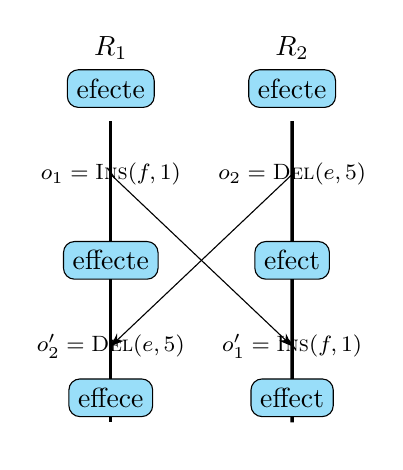
\begin{tikzpicture}[
	timeline/.style = {very thick}, >=Stealth, 
	send/.style = {>=Stealth, ->},
	list/.style = {rectangle, draw, rounded corners, fill = cyan!40, outer sep = 0pt},
	op/.style = {font = \footnotesize}
  ]
  \node[list, label = {above:{$R_1$}}] (r1) {efecte}; 
  \node[list, right = 1.20cm of r1, label = {above:{$R_2$}}] (r2) {efecte};

  \begin{scope}[on background layer]
    \foreach \r/\rbot in {r1/r1bot, r2/r2bot} {
      \node[below = 4.0cm of \r] (\rbot) {};
    }
  \end{scope}

  \draw[send] ($(r1)!0.25!(r1bot)$) node[op] (ins) {$o_1 = \ins{f}{1}$} to ($(r2)!0.75!(r2bot)$) node[op] () {$o_1' = \ins{f}{1}$};
  \draw[send] ($(r2)!0.25!(r2bot)$) node[op] (del) {$o_2 = \del{e}{5}$} to ($(r1)!0.75!(r1bot)$) node[op] () {$o_2' = \del{e}{5}$};

  \node (r11) [list] at ($(r1)!0.50!(r1bot)$) {effecte};
  \node (r12) [list] at ($(r1)!0.90!(r1bot)$) {effece};

  \node (r21) [list] at ($(r2)!0.50!(r2bot)$) {efect};
  \node (r22) [list] at ($(r2)!0.90!(r2bot)$) {effect};

  \draw[timeline] ($(r1.south)+(0,-5pt)$) -- (r11) -- (r12) -- (r1bot);
  \draw[timeline] ($(r2.south)+(0,-5pt)$) -- (r21) -- (r22) -- (r2bot);
\end{tikzpicture}
\end{document}
